% !TEX encoding = UTF-8 Unicode
\documentclass[a4paper,11pt]{article}
\usepackage[left=2cm,top=2.5cm,text={17cm,24cm}]{geometry}
\usepackage[utf8]{inputenc}
\usepackage[czech]{babel}
\usepackage[T1]{fontenc}
\usepackage{graphicx}
\usepackage{float}
\graphicspath{ {./images/} }

%========================= TITLE PAGE SETUP ===================================

\title{
\includegraphics[width=4.1cm,keepaspectratio,trim={1.2cm 1.2cm 1.2cm 1.2cm},clip]{vut-logo} \\
\vspace{4cm}
\textit{Simulační studie} \\
\textbf{Provoz chaty Triglavski dom na Krederici} \\
\vspace{0.5cm}
\textsc{IMS 2018/19 - FIT VUT, BRNO}}

\author{Dušek Vladimír (\textbf{xdusek27}), Andrej Naňo - \textbf{xnanoa00}}
\date{\today}

% big font for sections
\usepackage{sectsty}
\sectionfont{\LARGE}
\usepackage{url}
\usepackage{wrapfig}
\usepackage{caption}
\usepackage{subcaption}
\usepackage{listings}
% \usepackage{hyperref} % color
% \usepackage{dirtree}
% \usepackage{fontawesome}
\usepackage{listings}
\usepackage{color}
\usepackage{booktabs}
\usepackage{enumitem}
\usepackage{float}
\usepackage{amsmath}

%========================= SOURCE CODE STYLING ================================

\definecolor{bluekeywords}{rgb}{0.13,0.13,1}
\definecolor{greencomments}{rgb}{0,0.5,0}
\definecolor{redstrings}{rgb}{0.9,0,0}

\definecolor{gray}{rgb}{0.4,0.4,0.4}
\definecolor{darkblue}{rgb}{0.0,0.0,0.6}
\definecolor{cyan}{rgb}{0.0,0.6,0.6}

\lstset{
  basicstyle=\ttfamily,
  columns=fullflexible,
  showstringspaces=false,
  commentstyle=\color{gray}\upshape,
  captionpos=b
}

% == C language syntax hl ==
\lstdefinestyle{npl}{language=c,
  showspaces=false,
  showtabs=false,
  breaklines=true,
  showstringspaces=false,
  breakatwhitespace=true,
  escapeinside={(*@}{@*)},
  commentstyle=\color{greencomments},
  keywordstyle=\color{bluekeywords},
  stringstyle=\color{redstrings},
  basicstyle=\ttfamily,
  captionpos=b,
  numbers=left,
  frame=single,
  morekeywords={UINT8, UINT16, UINT32, INT8, INT16, INT32, Post, Properties, Protocol, AsciiString, String, StringTerm, BLOB, FormatString, this},
}

% == C++ language syntax hl ==
\lstdefinestyle{c++}{language=c,
  showspaces=false,
  showtabs=false,
  breaklines=true,
  showstringspaces=false,
  breakatwhitespace=true,
  escapeinside={(*@}{@*)},
  commentstyle=\color{greencomments},
  keywordstyle=\color{bluekeywords},
  stringstyle=\color{redstrings},
  basicstyle=\ttfamily,
  captionpos=b,
  numbers=left,
  frame=single,
  morekeywords={UINT8, UINT16, UINT32, INT8, INT16, INT32, Post, Properties, Protocol, AsciiString, String, StringTerm, BLOB, FormatString, this},
}

% \begin{comment} ... \end{comment{}
\usepackage{verbatim}

\setlength{\parskip}{0pt}

\makeatletter
\renewcommand{\paragraph}{
  \@startsection{paragraph}{4}
    {\z@}{1.25ex \@plus 1ex \@minus .2ex}{-1em}
      {\normalfont\normalsize\bfseries}
      }
      \makeatother

\usepackage{parskip}
\usepackage{lipsum}


%============================== TITLE PAGE ====================================

\begin{document}

\newpage
\maketitle
\newpage

%=========================== TABLE OF CONTENT =================================

\renewcommand{\contentsname}{Obsah}
\tableofcontents

%=============================== CONTENT ======================================

\section{Úvod}

V projektu jsme modelovali a simulovali\footnote{\url{https://www.fit.vutbr.cz/study/courses/IMS/public/prednasky/IMS.pdf}, slide 8} provoz horské chaty Triglavski Dom na Kredarici\footnote{\url{https://en.wikipedia.org/wiki/Triglav_Lodge_at_Kredarica}}. Jedná se o horskou chatu v Julských Alpách ve Slovinsku. Chata se nachází pod vrcholem hory Triglav ve výšce 2515\,m\,n.\,m. a tvoří záchytný bod pro většinu turistů, kteří se vydají horu zdolat.

Chata je kompletně odříznutá od civilizace, nedá se k ní dostat jinak než pěšky nebo vrtulníkem. Pochopitelně nevede k ní ani vedení zvlášť vysokého napětí. U chaty se nachází dvě větrné turbíny a společně se solárními panely na střeše jsou jediným zdrojem elektrické energie pro chatu a její návštěvníky. Ta se využívá na svícení, topení, provoz restaurace a podobně.\footnote{\url{https://www.summitpost.org/kredarica-hut-triglavski-dom-na-kredarici/349588}}

V práci se zabýváme produkcí energie těchto dvou zdrojů v daných podmínkách. Zvažujeme možná rizika technické závady elektráren, vliv nepříznivého počasí, či životnost akumulátorů. Na základě modelu\footnote{\url{https://www.fit.vutbr.cz/study/courses/IMS/public/prednasky/IMS.pdf}, slide 7} a simulačních experimentů\footnote{\url{https://www.fit.vutbr.cz/study/courses/IMS/public/prednasky/IMS.pdf}, slide 9} bude ukázán poměr produkce a výdeje energie. Z toho vyvodíme jak často hrozí, že by chata byla bez elektřiny. Ať už vlivem špatného počasí, technických problémů, či nadměrné spotřebě energie.

Smyslem experimentů je demonstrovat, že pokud by se přistavěli další zdroje energie, zvýšila by se kapacita akumulátorů, či by probíhali častější technické kontroly, tak by se zvýšila stabilita elektřiny.



\subsection{Autoři a zdroje informací}

Simulační studii vypracovali Vladimír Dušek a Andrej Naňo. Při tvorbě projektu byly využity znalosti nabyté v předmětu IMS. Pro zpracování modelu bylo nutné nastudovat princip větrných a fotovoltaických elektráren, zejména vliv počásí na jejich chod a akumulátory vhodné pro skladování energie z těchto zdrojů. Dále zjistit kolik turistů chatu během roku navštěvuje a jak je její provoz energeticky náročný. Informace jsme hledali na internetu, v každém odstavci jsou pak přesné odkazy na články, na jejich základě jsme danou informaci získali. Také jsme využili osobních zkušeností jednoho z autorů, který chatu navštívil.



\subsection{Ověřování validity modelu}

Problém validity modelu\footnote{\url{https://www.fit.vutbr.cz/study/courses/IMS/public/prednasky/IMS.pdf}, slide 10} jsme řešili konfrontací předpokládaných hodnot s hodnotami vystupujících z našeho simulačního modelu.
Vstupní hodnoty jsme optimalizovali na základě simulačních experimentů s modelem. Po dosáhnutí relativně uspokojivě přesných výsledků jsme systém prohlásili za dostatečně validní.

Verifikace modelů\footnote{\url{https://www.fit.vutbr.cz/study/courses/IMS/public/prednasky/IMS.pdf}, slide 36} proběhla v kapitole ~\ref{chap:mapping}, kde jsme ukázali mapování struktur/entit abstraktního modelu na třídy simulačního modelu.
      % Uvod do problematiky, proc danou studii provadime
\section{Rozbor tématu a použitých metod/technologií}\label{chap:analysis}

\subsection{Sumarizace faktů}



\subsubsection{Návštěvníci chaty}

Slovinské hory navštíví ročně kolem 1.7 milionu turistů.\footnote{\url{https://www.rtvslo.si/news-in-english/every-year-1-7-million-hikers-visit-slovenia-s-mountains/462870}}. Drtivá většina takto učiní v hlavní sezóně, období červen -- září. V době Slovinských prázdnin je pak špička úplně největší a na Triglav vystoupá až 2000 lidí za víkend.\footnote{\url{https://www.explore-share.com/blog/climbing-mount-triglav-slovenia/}} Po zbytek hlavní sezóny uvažujeme 1500 lidí za víkend. Ve všední dny pak počítáme s polovinou turistů. Délka hlavní sezóny jsou 4 měsíce (17 týdnů).

$8.5*2*1000=17000$\\
$8.5*5*500=21250$\\
$8.5*2*750=12750$\\
$8.5*5*375=15937$\\
$17000+21250+12750+15937=66937$\\
$66937/(17*7)=562$

V průběhu hlavní sezóny navštíví Triglav kolem \textbf{562} lidí denně. Mimo sezónu uvažujeme desetinu turistů, tedy \textbf{56} lidí denně.

Kapacita chaty pro přenocování je až \textbf{350} lidí. Restaurace může pojmout naráz zhruba \textbf{50} zákazníků.\footnote{\url{https://www.summitpost.org/kredarica-hut-triglavski-dom-na-kredarici/349588}}

Na úpatí hory jsou další dvě chaty, ty jsou ale podstatně menší a mají menší kapacitu. Předpokládáme, že Triglavski Dom navštíví \textbf{2/3} všech turistů. Na Triglav vede mnoho cest. Všechny jsou standardně dvoudenní, pouze velmi zkušení horolezci zvládnou celý výstup za jeden den.\footnote{\url{https://www.hedvabnastezka.cz/zeme/evropa/slovinsko/29363-vystup-na-triglav-cestou-cez-prag-trail/}} Jelikož Triglav je hora pro širší veřejnost, uvažujeme, že pro přenocování se rozhodne \textbf{4/5} turistů. Ty na chatě zůstanou dobu definovanou normálním rozdělením se středem \textbf{12} hodin. Zbytek se na chatě zastaví pouze krátce, dobu definovanou normálním rozdělením se středem \textbf{3} hodiny.

Bereme v potaz i situaci, kdy by na chatě nešla elektřina. To by znamenalo značné omezení fungovaní restaurace a hlavně zimu. Předpokládáme, že by to malé množství návštěvníků chaty odradilo. Buď by se na základě toho rozhodli pro jednodenní výstup, využili by služeb jiné chaty, nebo se vrátili zpět do údolí. Takto by se podle našich odhadů zachovalo \textbf{10\%} zákazníků.



\subsubsection{Spotřeba energie}

Na základě grafu\footnote{\url{https://www.statista.com/statistics/195728/average-energy-consumption-per-guest-night-in-hotels-by-continent/}} jsme určili spotřebu energie hosta za noc. Bude se řídit normálním rozdělením se středem \textbf{20\,kWh} (70MJ). Bereme výrazně nižší hodnotu, než je průměr, protože se jedná o horskou chatu, ne standardní hotel. U návštěvníků, kteří se zastaví pouze na kratší odpočinek bude spotřeba velmi nízká a uvažujeme normální rozložení se středem \textbf{5\,kWh} (70MJ).

Chata sama o sobě spotřebuje nějakou energii, i bez zákazníků. Například topit a svítit se bude do jisté míry i pro personál. Průměrný americký hotel spotřebuje 14\,kWh na $ft^2$ ročně.\footnote{\url{https://www.mge.com/saving-energy/business/bea/article_detail.htm}} Na základě této úměry odhadujeme spotřebu naší chaty na \textbf{180\,kWh} denně.



\subsubsection{Větrné turbíny}

Větrné turbíny začínají produkovat energii při rychlosti větru 4 až 5 metrů za sekundu a maximálního výkonu dosahují při rychlosti 15 metrů za sekundu. Naopak při velmi silném větru nad 25 metrů za sekundu se turbíny vypínají.\footnote{\url{http://www.ewea.org/wind-energy-basics/faq/}} Na základě informací z\footnote{\url{https://www.engineering.com/ElectronicsDesign/ElectronicsDesignArticles/ArticleID/9556/Rooftop-Wind-Turbines-Are-They-Worthwhile.aspx}} \footnote{\url{https://www.meteoblue.com/en/weather/forecast/modelclimate/kredarica_slovenia_3197311}} jsme sestavili tabulku~\ref{tab:wind_energy} produkce energie turbíny dle síly větru.

\begin{center}
    \begin{table}[!h]
        \centering
        \begin{tabular}{|c|c|}
            \hline
            Síla větru [km/hod] & Produkce energie jedné turbíny [$kWh/$hod] \\
            \hline
            \hline
            0 - 4.5 & 0 \\
            \hline
            4.5 - 10 & 0.1 \\
            \hline
            10 - 20 & 0.2 \\
            \hline
            20 - 30 & 0.4 \\
            \hline
            30 - 54 & 0.8 \\
            \hline
            54 - 90 & 1 \\
            \hline
            90 + & 0 \\
            \hline
        \end{tabular}
        \caption{Produkce energie vetrné turbíny v závislosti na síle větru}
        \label{tab:wind_energy}
    \end{table}
\end{center}

Sílu větru v naší lokalitě generujeme jako normální rozložení se středem 40\,km/hod.

Větrná turbína je odstavena kvůli technickým závadám v průměru 170 hodin za rok. \footnote{\url{https://www.nrel.gov/docs/fy13osti/59111.pdf}}



\subsubsection{Fotovoltaické panely}

Pomocí Google Maps jsme naměřili rozměry chaty.\footnote{\url{https://goo.gl/maps/Mey2s4gSWC82}} Ty činí $30\,m * 23\,m * 10\,m$. Dále jsme usoudili, že průměrná výška střechy (není z obou stran stejná) může být 6m. Vypočítali jsme druhý rozměr střechy $\sqrt{9^{2}+6^{2}} \approx 10.8\,m$. Z těchto rozměrů jsme už vypočítali celkovou plochu střechy $2*10.8*24 \approx 518\,m^2$. Z obrázků chaty jsme usoudili, že solární panely mohou být nainstalovány zhruba na 3/4 střechy.\footnote{\url{https://goo.gl/images/nLK9Lp}} Celkově tedy máme {\boldmath$389\,m^2$} solárních panelů. Solární panely mají průměrně velikost $165\,cm * 99\,cm \approx 16.3\,m^2$ \footnote{\url{https://www.solarpowerrocks.com/solar-basics/how-much-electricity-does-a-solar-panel-produce/}} Na střeše chaty se tedy nachazí asi \textbf{24} solárních panelů.

\begin{figure}[H]
    \centering
    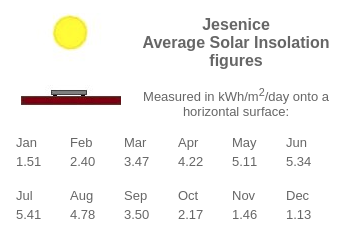
\includegraphics[width=.40\textwidth]{images/solar_energy.png}\hfill
    \caption{Produkovaná energie solárních panelů}
    \label{fig:solar_energy}
\end{figure}

Na obrázku~\ref{fig:solar_energy} je zachycena produkce energie solárních panelů na základě geografické polohy a jejich nasměrování vůči Slunci.\footnote{\url{http://solarelectricityhandbook.com/solar-irradiance.html?fbclid=IwAR0W-VqbCV1noK_vQZl4-U8a4ibCUvSwaAoGB0Nu52Dbzsnx_cmy2JlQMKU}} Na základě těchto dat, jsme spočítaly produkci energie všech panelů dle měsíců v roce.

\begin{center}
    \begin{table}[H]
        \centering
        \begin{tabular}{|c|c|}
            \hline
            Měsíc & Produkce energie jednoho panelu [$Kwh/$den] \\
            \hline
            \hline
            leden & 24.6 \\
            \hline
            únor & 39.1 \\
            \hline
            březen & 56.6 \\
            \hline
            duben & 68.8 \\
            \hline
            květen & 83.3 \\
            \hline
            červen & 87 \\
            \hline
            červenec & 88.2 \\
            \hline
            srpen & 77.9 \\
            \hline
            září & 57 \\
            \hline
            říjen & 35.4 \\
            \hline
            listopad & 23.8 \\
            \hline
            prosinec & 18.4 \\
            \hline
        \end{tabular}
        \caption{Produkce energie solárních panelů v závislosti na měsíci}
    \end{table}
\end{center}

Poruchovost solárních panelů je velmi nízka, v průměru 0.05\%. Jednou z hlavních příčin ovčem je silný vítr.\footnote{\url{https://news.energysage.com/average-solar-panel-failure-rate/}} My se ovšem nacházíme v lokalitě kde je vítr extrémně silný, budeme tedy uvažovat až 4x větší poruchovost, tedy \textbf{0.2\%}.\footnote{\url{http://www.meteocentrale.ch/en/europe/slovenia/weather-kredarica/details/S140080/}} Výměna solárního panelu by mohla trvat řádově měsíce, uvažujeme \textbf{3}.



\subsubsection{Akumulátory}

Skladování energie není úplně snadná záležitost. Uvažujeme, že \textbf{9/10} energie co uložíme budeme moci opět využít.\footnote{\url{https://www.energysage.com/solar/solar-energy-storage/what-are-the-best-batteries-for-solar-panels/}} Velikost akumulátorů v chatě odhadujeme celkem na \textbf{5000\,kWh}.\footnote{\url{https://www.wholesalesolar.com/solar-information/battery-bank-sizing}}



\subsection{Použité postupy pro vytvoření modelu a původ použitých metod/technologií}

Pro tvorbu simulačního modelu byl použit jazyk C++ s knihovnou SIMLIB.
\begin{itemize}
    \item C++\\
    \url{http://www.cplusplus.com/}
    \item SIMLIB\\
    \url{http://www.fit.vutbr.cz/~peringer/SIMLIB/}
\end{itemize}

Použité konstrukce a algoritmy jsou převážně inspirovány studijními materiály předmětu IMS.
\begin{itemize}
    \item IMS prezentace\\
    \url{https://www.fit.vutbr.cz/study/courses/IMS/public/prednasky/IMS.pdf}
    \item První democvičení\\
    \url{http://perchta.fit.vutbr.cz:8000/vyuka-ims/uploads/1/ims-demo1.pdf}
    \item Druhé democvičení\\
    \url{http://perchta.fit.vutbr.cz:8000/vyuka-ims/uploads/1/diskr2-2011.pdf}
    \item Dokumentace SIMLIB\\
    \url{http://www.fit.vutbr.cz/~peringer/SIMLIB/doc/SimLib-doc-2.ps}
    \item Doxygen dokumentace SIMLIB\\
    \url{https://www.fit.vutbr.cz/~peringer/SIMLIB/doc/html/}
    \item Příklady SIMLIB
    \url{http://www.fit.vutbr.cz/~peringer/SIMLIB/examples/}
\end{itemize}
          % Rozbor tematu, shrnuti faktu
\section{Koncepce}

V následující kapitole je definován konceptuální model\footnote{\url{https://www.fit.vutbr.cz/study/courses/IMS/public/prednasky/IMS.pdf}, slide 48}, který jsme vytvořili na základě faktů systému představených v předcházející kapitole. Na základě konceptuálního modelu jsme následně vytvořili model simulační\footnote{\url{https://www.fit.vutbr.cz/study/courses/IMS/public/prednasky/IMS.pdf}, slide 44}.



\subsection{Způsob vyjádření konceptuálního modelu}

Následující schéma prezentuje systém jako celek. Tento systém budeme dále dělit na podsystémy a modelovat pomocí Petriho sítí\footnote{\url{https://www.fit.vutbr.cz/study/courses/IMS/public/prednasky/IMS.pdf}, slide 123}.

\begin{figure}[H]
    \centering
    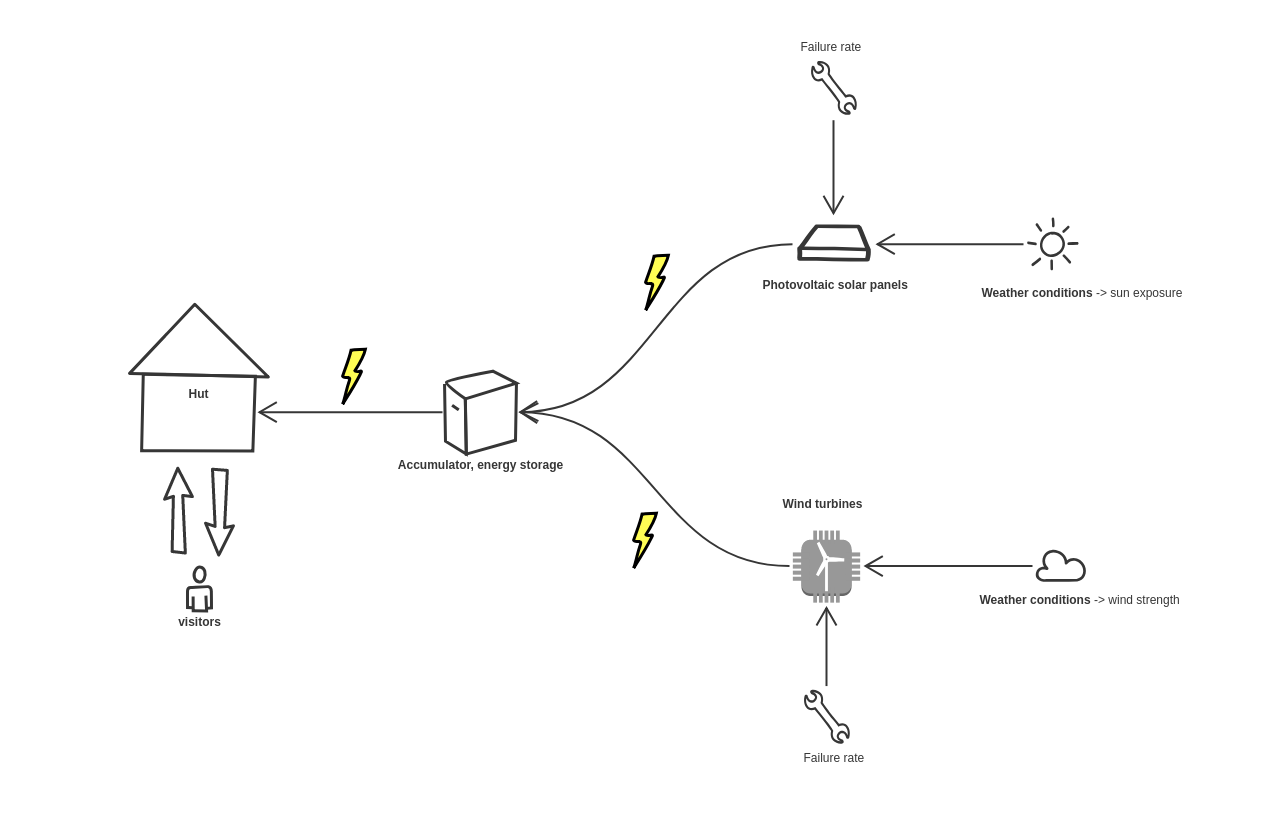
\includegraphics[width=.99\textwidth]{images/schema.png}\hfill
    \caption{Schéma systému}
    \label{fig:schema}
\end{figure}



\subsection{Forma konceptuálního modelu}

Na dalších obrázcích jsou zachyceny jednotlivé podsystémy modelované Petriho sítí.

\begin{figure}[H]
    \centering
    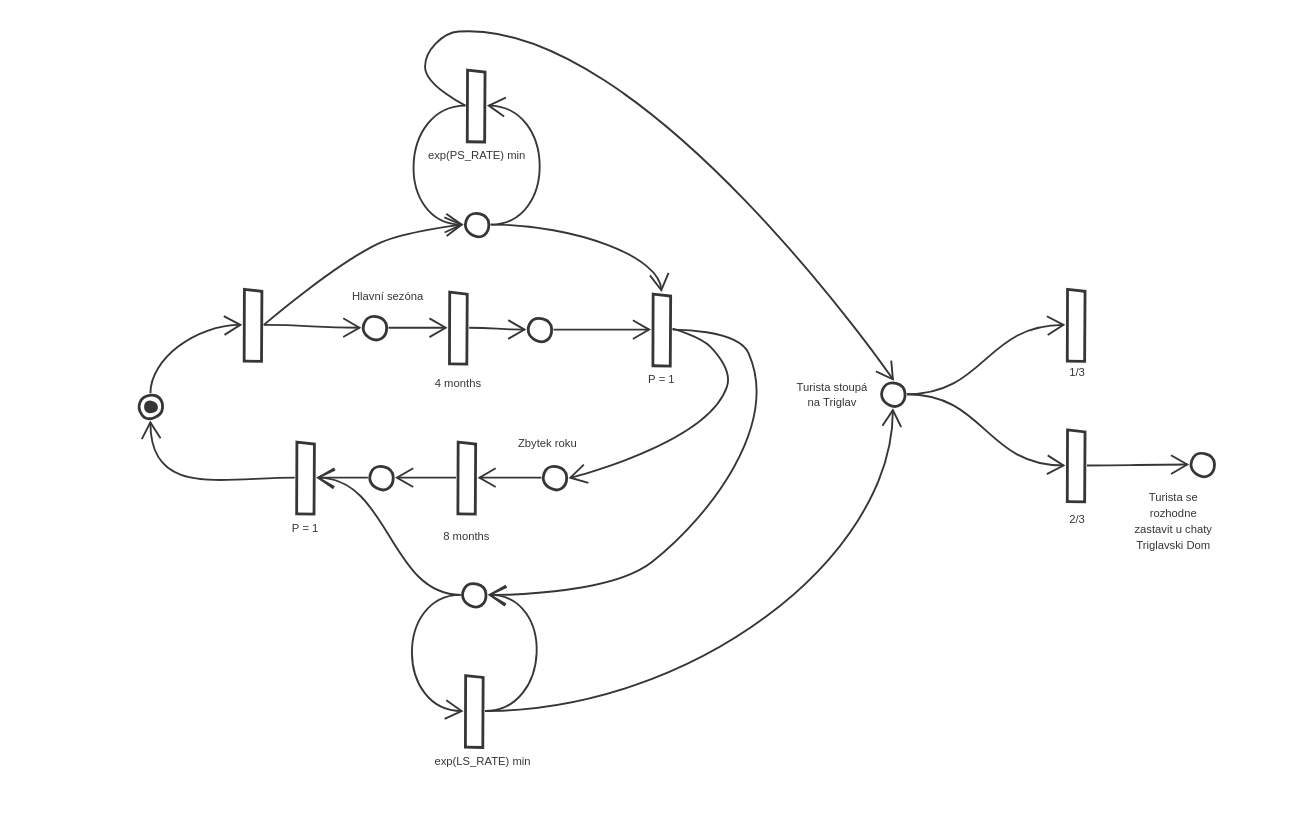
\includegraphics[width=.99\textwidth]{images/petri_net_visitors.png}\hfill
    \caption{Generování turistů}
    \label{fig:petri_net_visitors}
\end{figure}

\begin{figure}[H]
    \centering
    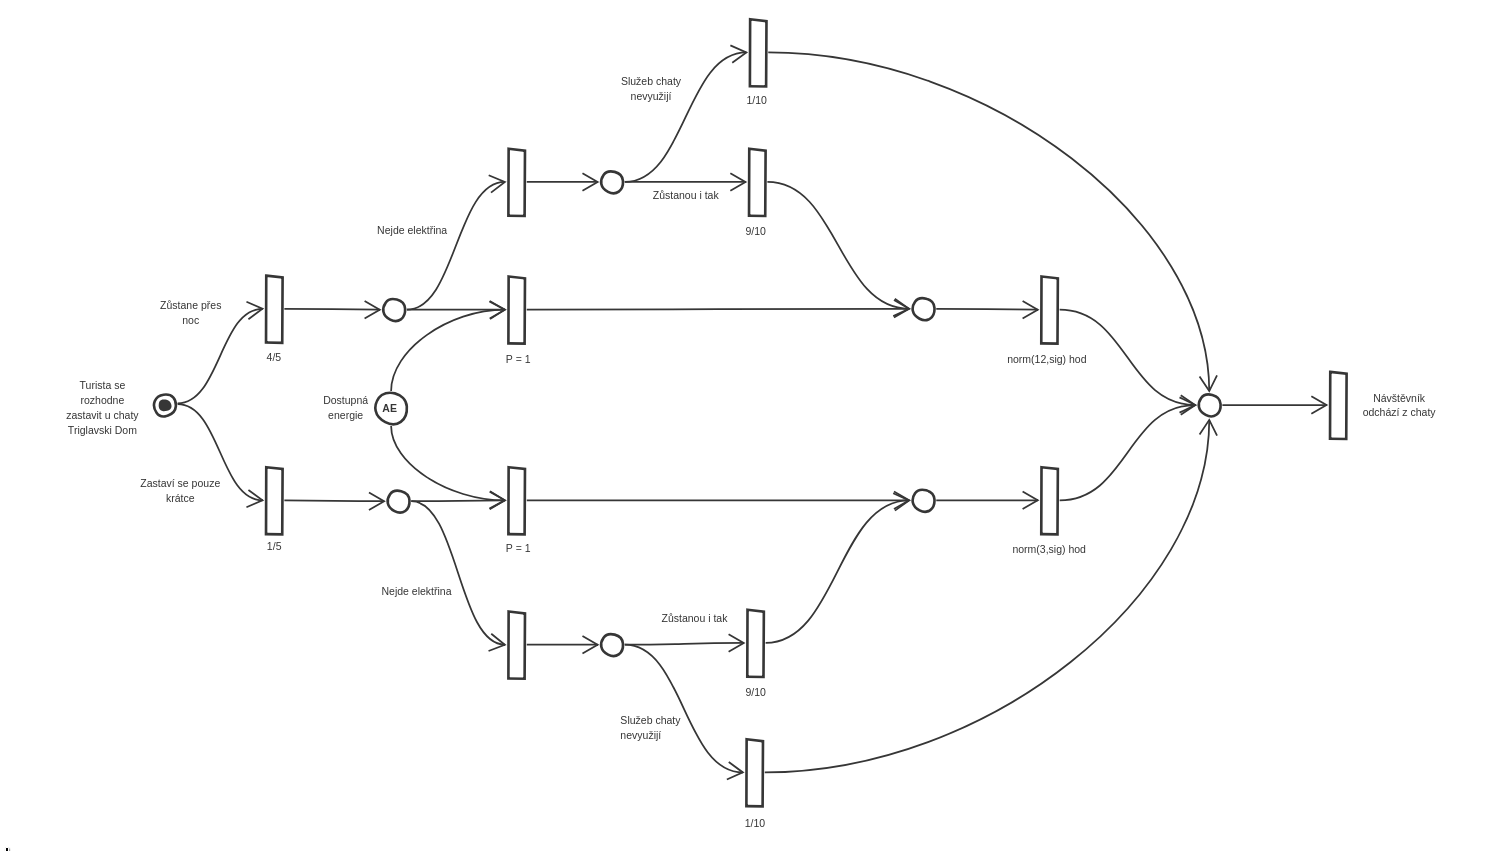
\includegraphics[width=.99\textwidth]{images/petri_net_visitor_in_hut.png}\hfill
    \caption{Návštěvník v chatě}
    \label{fig:petri_net_visitor_in_hut}
\end{figure}

\begin{figure}[H]
    \centering
    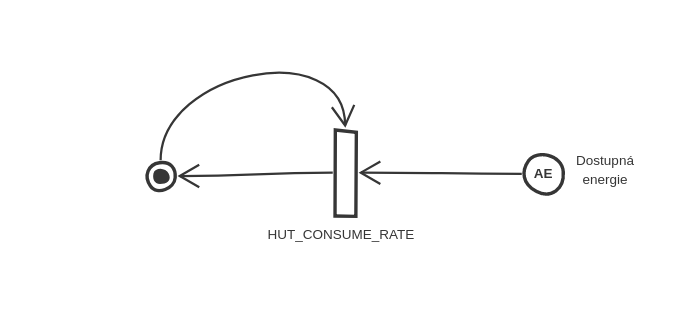
\includegraphics[width=.5\textwidth]{images/petri_net_hut.png}\hfill
    \caption{Energie potřebná pro základní chod chaty}
    \label{fig:petri_net_hut}
\end{figure}

\begin{figure}[H]
    \centering
    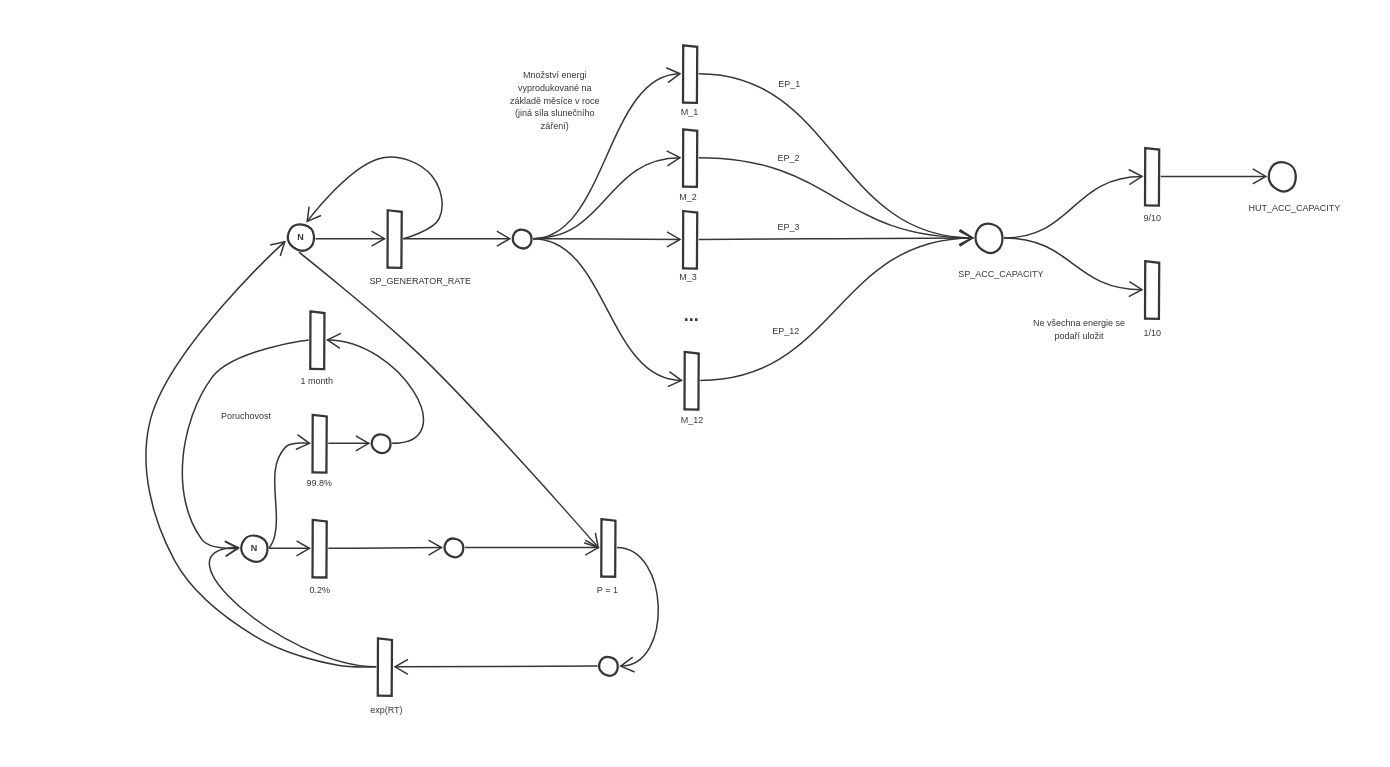
\includegraphics[width=.99\textwidth]{images/petri_net_solar_energy.png}\hfill
    \caption{Energie generovaná solárními panely}
    \label{fig:petri_net_solar_energy}
\end{figure}

\begin{figure}[H]
    \centering
    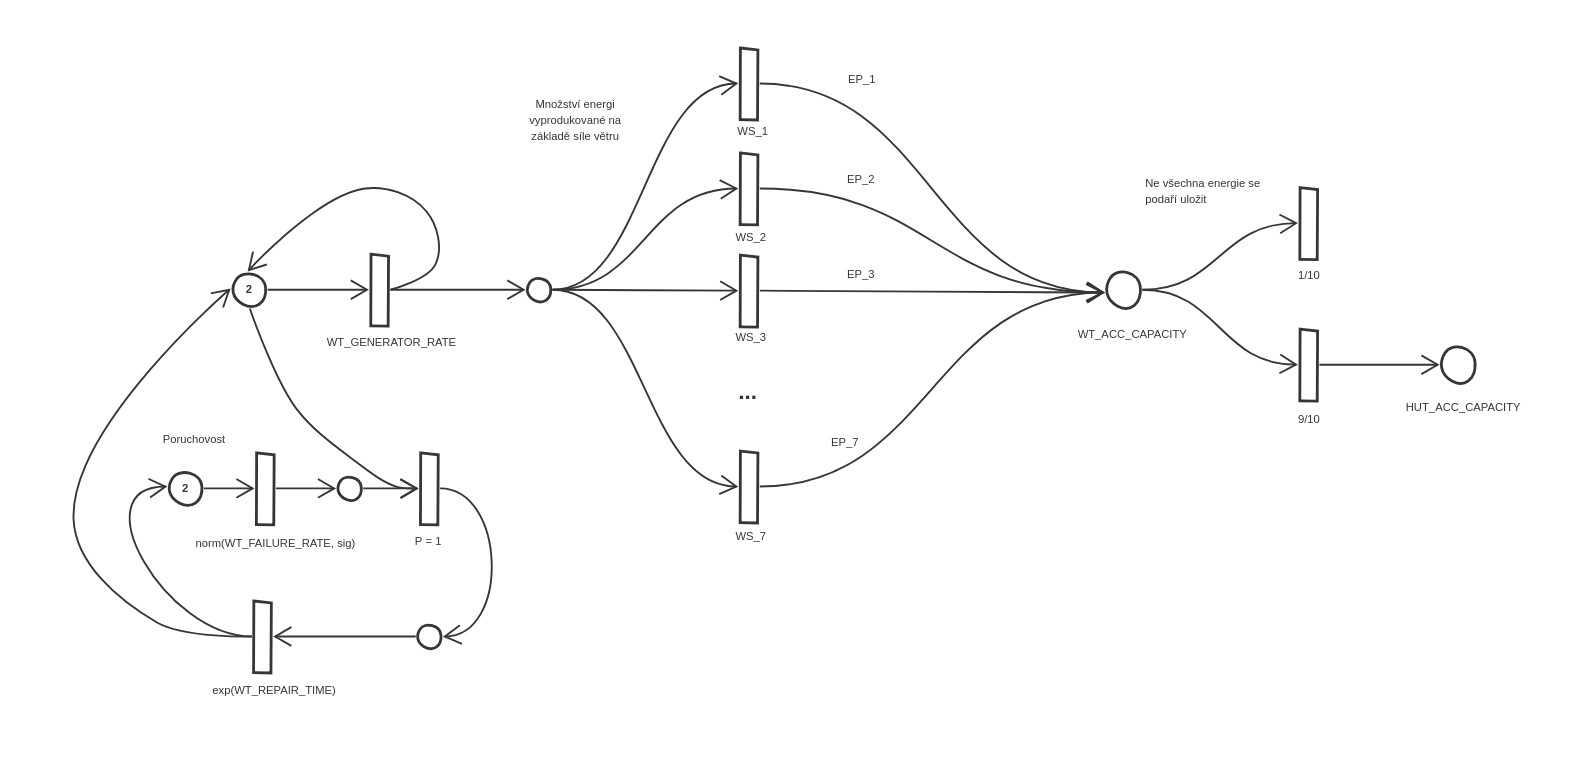
\includegraphics[width=.99\textwidth]{images/petri_net_wind_energy.png}\hfill
    \caption{Energie generovaná větrnými turbínami}
    \label{fig:petri_net_wind_energy}
\end{figure}
        % Koncepce modelu, abstraktni model
\section{Architektura simulačního modelu}\label{chap:mapping}

\subsection{Mapování konceptiálního modelu na simulační}

V tabulce~\ref{tab:map_con_sim} je zobrazeno mapování jednotlivých entit konceptuálního modelu na třídy simulačního modelu.

\begin{center}
    \begin{table}[!h]
        \centering
        \begin{tabular}{|c|c|}
            \hline
            Entita v konceptuálním modelu & Třída v simulačním modelu \\
            \hline
            \hline
            Transakce změny sezóny & SeasonChange \\
            \hline
            Transakce návštěvníka & Visitor \\
            \hline
            Transakce energie větrné turbíny & WT\_Energy \\
            \hline
            Transakce chyby větrné turbíny & WT\_Failure \\
            \hline
            Transakce energie solárního panelu & SP\_Energy \\
            \hline
            Transakce chyba solárního panelu & SP\_Failure \\
            \hline
            Přesun energie z akumulátoru do chaty & EnergyFlow \\
            \hline
            Transakce fungování chaty & Hut \\
            \hline
            Generátor návštěvníků v hlavní sezóně & PeakSeasonVisitorGenerator \\
            \hline
            Generátor návštěvníků mimo hlavní sezónu & LowSeasonVisitorGenerator \\
            \hline
            Generátor energie z větrné turbíny & WindTurbineGenerator \\
            \hline
            Generátor poruchy větrné turbíny & WindTurbineFailureGenerator \\
            \hline
            Generátor energie ze solárního panelu & SolarPanelsGenerator \\
            \hline
            Generátor poruchy solárního panelu & SolarPanelsFailureGenerator \\
            \hline
            Generátor využívání energie chatou & EnergyUsageGenerator \\
            \hline
            Přesunutí energie do akumulátoru & FlowGenerator \\
            \hline
            \hline
        \end{tabular}
        \caption{Mapování konceptuálního modelu na simulační}
        \label{tab:map_con_sim}
    \end{table}
\end{center}


      % Architektura simulacniho modelu
\section{Podstata simulačních experimentů a jejich průběh}

Cílém experimentů bylo zjistit jak často je chata bez energie a o kolik se tím potenciálně připravujeme zákazníků. Dále jaké jsou možnosti řešení dobu bez energie minimalizovat. Ať už přistavěním dalšího zdroje energie, či zvýšením kapacity akumulátorů.



\subsection{Postup experimentování}

Nejprve simulujeme provoz chaty s údaji které maximálně odrážejí současnost pro několik let běžného provozu. Můžeme se zaměřit pouze na hlavní sezónu, kdy je nápor největší. Hrozí nejvíce výpadků energie a taky mají nejhorší následky, přicházíme o zákazníky. Analyzujeme potenciální ztrátu zákazníků, dobu po kterou jsou akumulátory zaplněné a dobu po kterou jsme bez energie.

Pro další experimentování jsme zvýšili počet větrných turbín a přistavěli další solární panely, střecha chaty není úplně zaplněná.



\subsection{Jednotlivé experimenty}

\subsection{Prvotní experimenty}

Na základě statistik~\ref{tab:res_1} z prvního experimentu jsme zjistili, že náš model dává podivné výsledky při generování energie. Konkrétně, že jediný solární panel generuje daleko více energie než jedna větrná turbína. Pravděpodobně jsme udělali někde chybu při sbírání faktů. Generování energie větrnou turbínou jsme zvýšili.

\begin{figure}[H]
    \begin{verbatim}
    +----------------------------------------------------------+
    | STATISTIC Energy generated by wind turbines              |
    +----------------------------------------------------------+
    |  Min = 0                       Max = 83                  |
    |  Number of records = 210240                              |
    |  Average value = 48.7062                                 |
    |  Standard deviation = 17.6815                            |
    +----------------------------------------------------------+
    +----------------------------------------------------------+
    | STATISTIC Energy generated by solar panels               |
    +----------------------------------------------------------+
    |  Min = 63                      Max = 306                 |
    |  Number of records = 2522880                             |
    |  Average value = 190.573                                 |
    |  Standard deviation = 87.0823                            |
    +----------------------------------------------------------+
    \end{verbatim}
    \caption{Výsledky experimentu 1}
    \label{tab:res_1}
\end{figure}

Na základě statistik~\ref{tab:res_2} z druhého experimentu jsme zjistili, že zákazníci si berou příliš mnoho energie. Pravděpodobně jsme špatně odhadli spotřebu na zákazníka, kterou jsme zakládali na průměrné spotřebě hotelů (viz kapitola ~\ref{chap:analysis}). Spotřebu návštěvníků jsme snížili na 4.5\,kWh pro noc a 1.0\,kWh pro den.

\begin{figure}[H]
    \begin{verbatim}
        +----------------------------------------------------------+
        | STATISTIC Number of guests in the hut at the same time   |
        +----------------------------------------------------------+
        |  Min = 1                       Max = 185                 |
        |  Number of records = 525600                              |
        |  Average value = 54.3021                                 |
        |  Standard deviation = 58.6799                            |
        +----------------------------------------------------------+
        +----------------------------------------------------------+
        | STATISTIC Energy need per visitor                        |
        +----------------------------------------------------------+
        |  Min = 0                       Max = 6369.79             |
        |  Time = 0 - 3.1536e+10                                   |
        |  Number of records = 49404                               |
        |  Average value = 1625.7                                  |
        +----------------------------------------------------------+
        +----------------------------------------------------------+
        | STATISTIC Visitors per day                               |
        +----------------------------------------------------------+
        |  Min = 18                      Max = 414                 |
        |  Number of records = 365                                 |
        |  Average value = 135.353                                 |
        |  Standard deviation = 145.575                            |
        +----------------------------------------------------------+
    \end{verbatim}
    \caption{Výsledky experimentu 2}
    \label{tab:res_2}
\end{figure}


Na základě grafu z obrázku~\ref{fig:graph_1} jsme zjistili, že v půlce hlavní seźony energie dojde a již se ji nepodaří doplňovat. Půlku sezóny tedy bude chata kompletně bez energie. Mimo hlavní sezónu je výdaj výrazně nižší, proto dostupná energie bude téměř stále na maximu.


\begin{figure}[H]
    \centering
    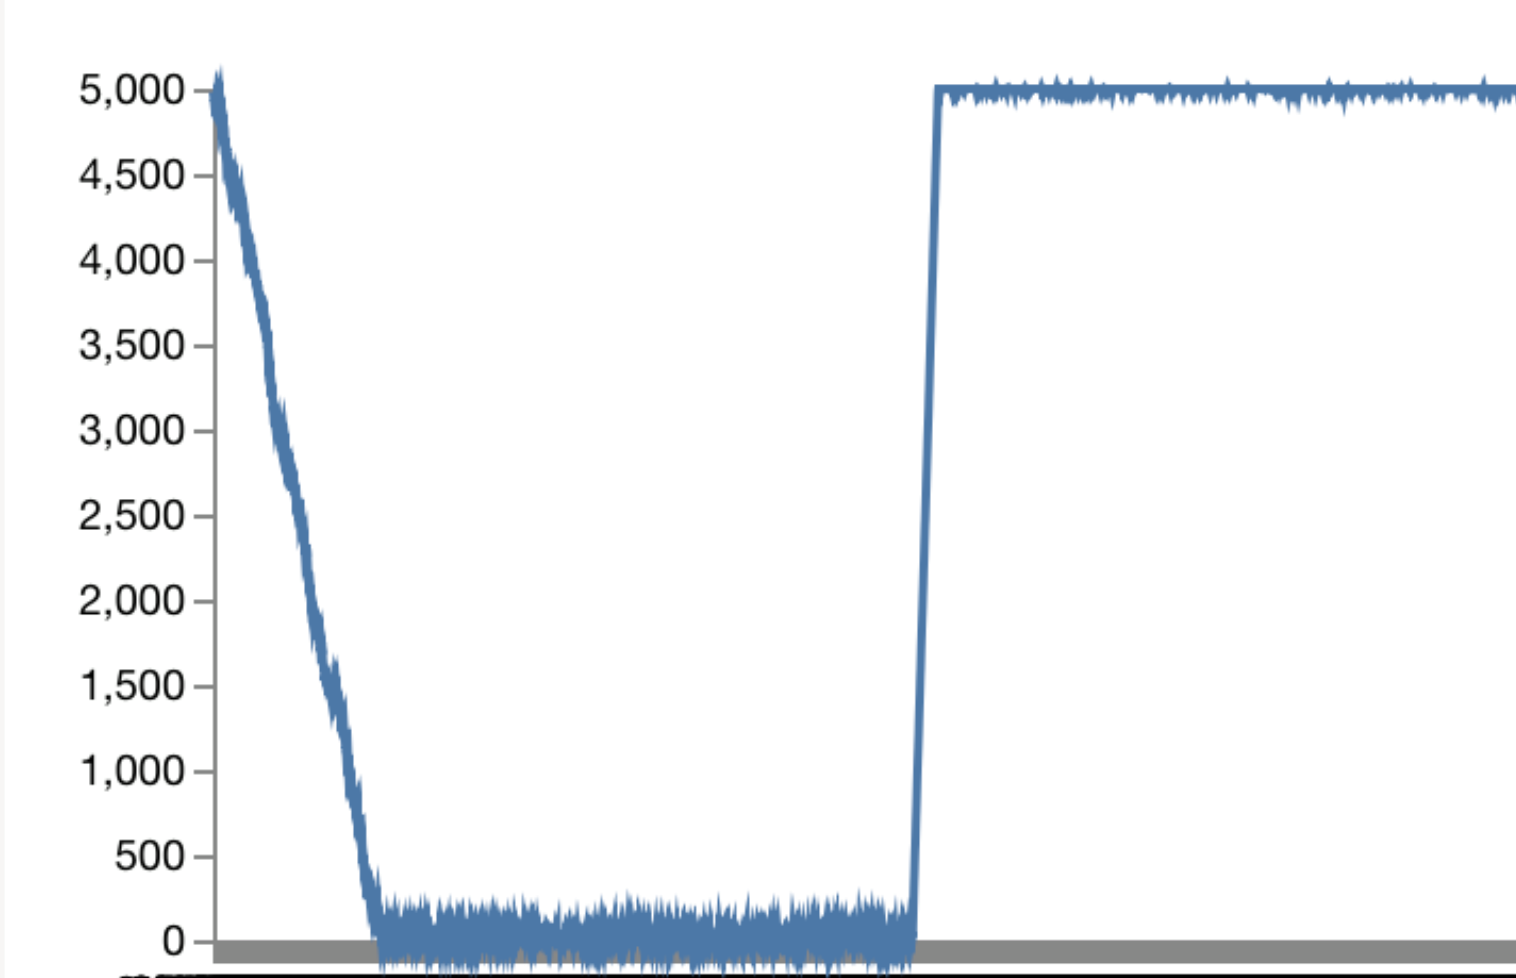
\includegraphics[width=.75\textwidth]{images/graph_1.png}\hfill
    \caption{Množství energie v průběhu roku}
    \label{fig:graph_1}
\end{figure}



\subsubsection{Přidání větrné turbíny}

Stav v případě, že bychom se rozhodli postavit další větrnou turbínu je zachycen na obrázku~\ref{fig:graph_2}. Přistavění větrné turbíny by situaci vyřešilo pouze částěčně.

\begin{figure}[H]
    \centering
    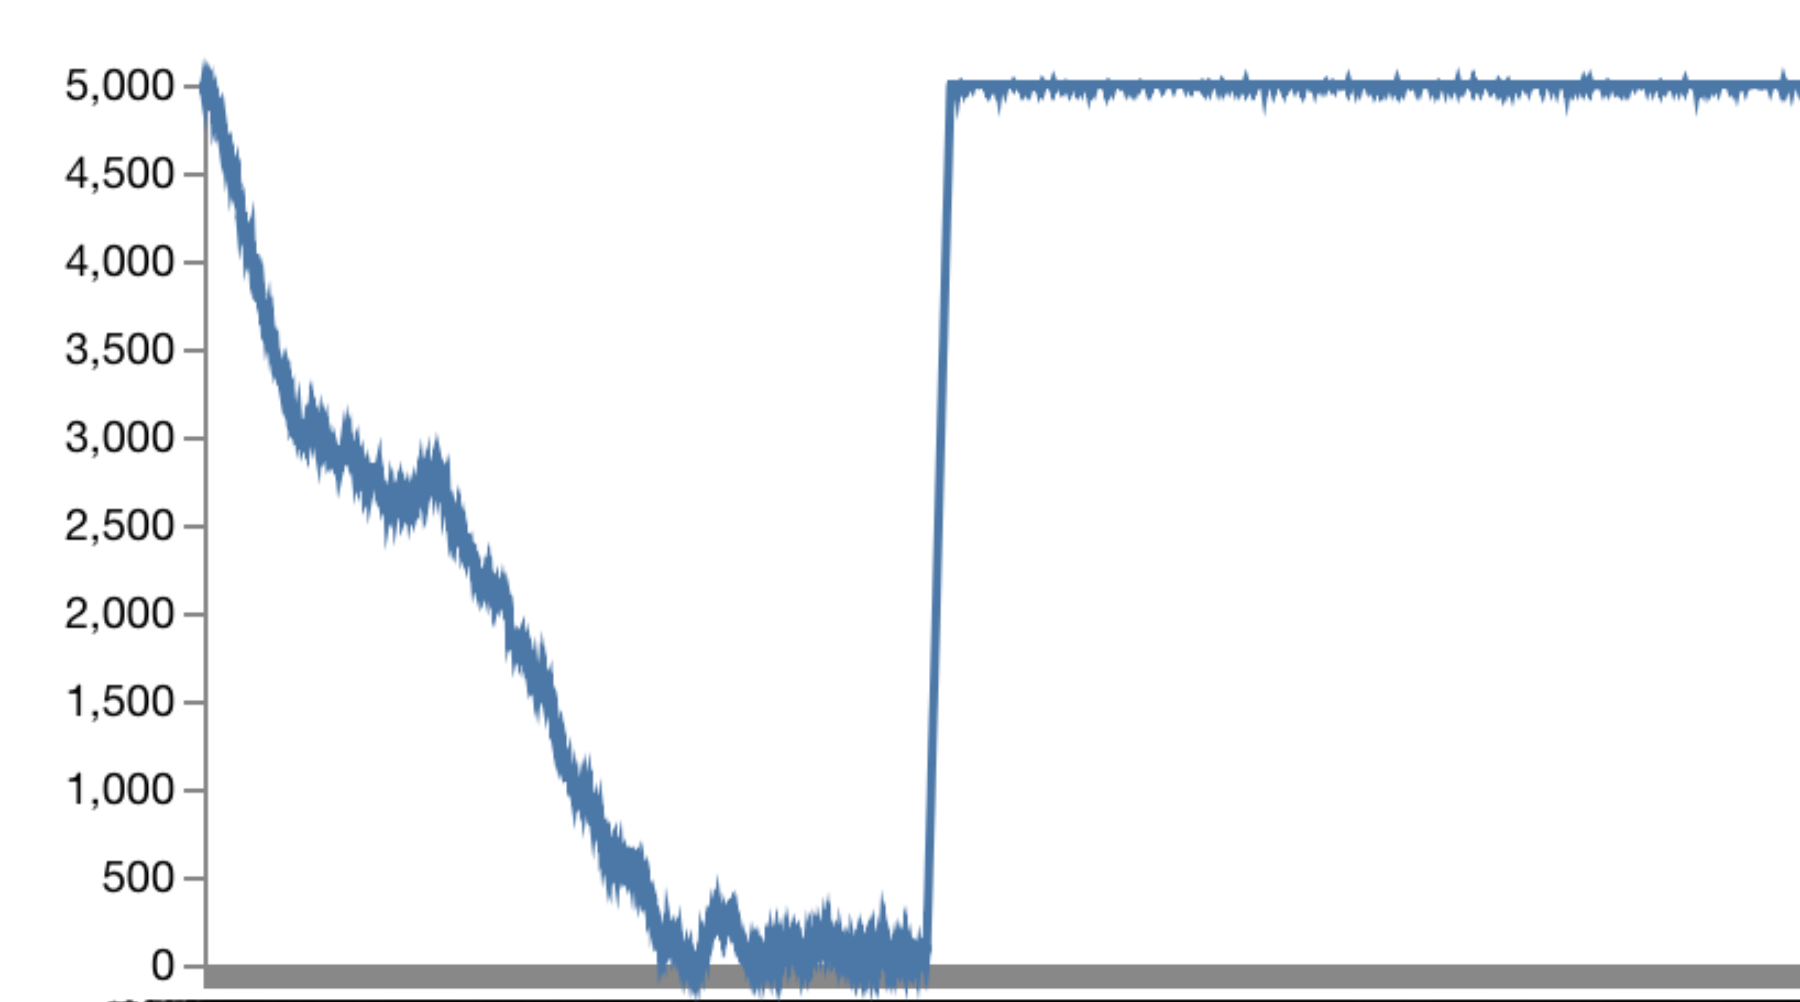
\includegraphics[width=.75\textwidth]{images/graph_2.png}\hfill
    \caption{Množství energie v průběhu roku (+1 turbína)}
    \label{fig:graph_2}
\end{figure}


\subsubsection{Přidání ještě solárních panelů}

Stav v případě, že bychom se rozhodli přidat ještě jeden solární panel je zachycen na obrázku~\ref{fig:graph_3}. Vidíme, že přistavět jeden panel stačí a situace je vyřešena. Chata bude mít stabilně energii po celý rok.

\begin{figure}[H]
    \centering
    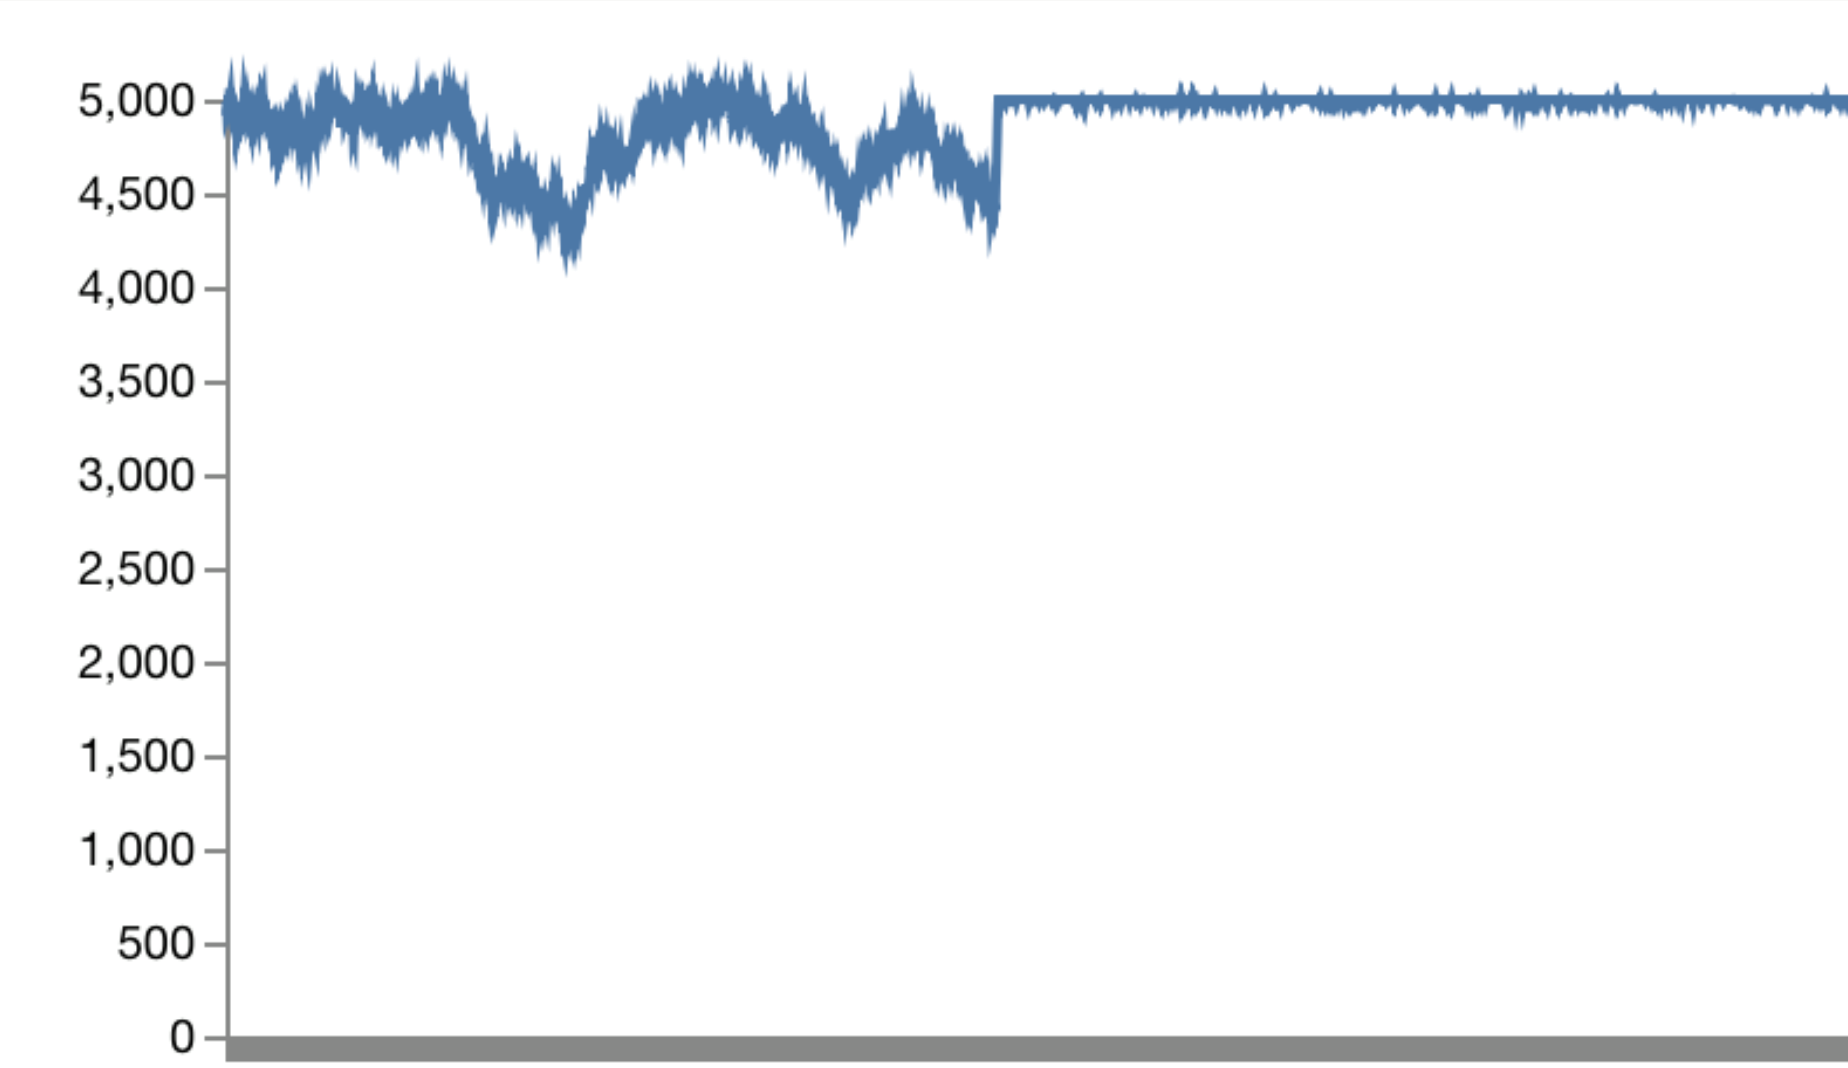
\includegraphics[width=.75\textwidth]{images/graph_3.png}\hfill
    \caption{Množství energie v průběhu roku (+1 turbína a +1 panel)}
    \label{fig:graph_3}
\end{figure}


\subsection{Závěr experimentování}

Z experimentů jsme zjistili, že naše posbíraná data nemusela být naprosto korektní. Někde došlo k nějaké nepřesnosti a nejprve nám vycházeli nesmysli. Postupně jsme upravovali produkci energie větrnou turbínou a spotřebu návštěvníka chaty.

Na dalších experimentech jsme se zjišťovali přidávání zdrojů energie. Ideální případ by byl přistavět jednu větrnou turbínu a jeden solární panel. Již to by stačilo pro zajištění stability energie po celý rok.
           % Podstata simulacnich experimentu, co chceme zjistit
\section{Shrnutí simulačních experimentů a závěr}

Na simulačním modelu jsme prováděli řadu experimentů. Nejprve jsme vyladili hodnoty, díky kterým jsme model přivedli do validního stavu. Větrné turbíny produkovali velmi málo energie a spotřeba zákazníka chaty byla nereálně vysoká, na což jsme přišly na základě experimentování. Dalším experimentováním jsme zjistili potenciální možnosti udržení stability energie na chatě a tím se vyhnout ztrátám energie a tím i ztrátám zákazníků.

V rámci projektu vzikl simulační nástroj pro provoz horské chaty. Dalšími bychom mohli například zjišťovat z ekonomického aspektu, či se nám vyplatí stavět další solární panely, či větrné turbíny. Dale například či by se vyplatilo zvyšovat kapacitu chaty.
           % Shrnuti experimentu, zavery, vysledky

\end{document}
